\documentclass{article}
\usepackage{iclr2027_conference,times}
\usepackage{amsmath,amssymb}
\usepackage{booktabs}
\usepackage{graphicx}
\usepackage{microtype}
\usepackage{hyperref}
\usepackage{url}

\title{OrbitCover: Interaction-Balanced Estimation\\
of Semantic Predictor Quotients}

% Keep \iclrfinalcopy commented out for the anonymous submission.
\author{Anonymous authors}

\newcommand{\E}{\mathbb{E}}
\newcommand{\Qhat}{\widehat{Q}}

\begin{document}
\maketitle

\begin{abstract}
Two tables can encode the same supervised problem while differing only in
feature order, opaque category identifiers, or target identifiers. A learning
pipeline need not return the same predictor on these equivalent
representations, and ordinary seed ensembling does not integrate over this
larger nuisance space. We formulate the output of a randomized learning
pipeline as a vector-valued function on a declared finite product of semantic
symmetries and training randomness. Its orbit average is a \emph{quotient
predictor}. For Brier and squared loss, prediction variance around this
quotient is exactly the expected finite-member loss overhead. Product
functional ANOVA (fANOVA) makes its source observable. OrbitCover applies a
randomized mixed-level orthogonal array to the complete train-and-predict
pipeline: a strength-$t$ design cancels every fANOVA component of order at
most $t$. We evaluate 12 datasets, three splits, and four neural architectures
(144 primary cells). At $B=16$, the coupled strength-2 construction has lower
method-relative residual than canonical independent ensembling in 144/144
cells and 12/12 datasets, with a dataset-balanced reduction of 55.9\% and a
dataset-clustered 95\% interval of [38.7\%, 73.8\%]. This is not a
same-estimand comparison: the canonical and symmetrized expectations are
measurably distinct in 10/144 cells. A 48-cell same-target ablation attributes
a 47.6\% mean cellwise reduction to jointly balancing schema, initialization,
and training order. Fresh independent randomness removes the schema-only
benefit ($-7.0$\% versus canonical independent), and the strength-2 advantage
over simple random sampling vanishes on average at convergence (residual ratio
1.002). OrbitCover is therefore an auditable finite-budget estimator for a
declared semantic quotient, not a universally better ensemble.
\end{abstract}

\section{Introduction}

Tabular models receive an array, but users intend a statistical problem.
Reordering feature blocks, bijectively renaming opaque categories, or swapping
class identifiers together with their decoding leaves that problem unchanged.
The implementation path is less abstract: positional parameters, random
initialization, batching, dropout, and finite optimization can couple to the
chosen representation. Two legitimate executions can therefore produce
different \emph{aligned} predictions.

Recent tabular work has made models stronger and evaluation broader. TabM
studies parameter-efficient neural ensembling \citep{gorishniy2025tabm};
TabPFN-v2 performs in-context prediction with a learned prior
\citep{hollmann2025tabpfn}; TabDPT and TabSTAR develop foundation-style
tabular prediction \citep{ma2025tabdpt,arazi2025tabstar}; and TabArena and
TabReD emphasize reproducible, realistic evaluation
\citep{erickson2025tabarena,rubachev2025tabred}. These advances sharpen a
basic question: \emph{which randomized predictor is a reported score intended
to describe?} Several seeds of one canonical encoding target only one slice
of the pipeline. Averaging arbitrary schema transformations is also incomplete
unless outputs are aligned and the sampling law is declared.

We define the target first. A finite nuisance product $\Omega$ contains exact
schema transformations and stochastic choices of the complete learning
pipeline. After semantic alignment, its prediction barycenter is the quotient
predictor. Estimating it is finite-dimensional integration of an expensive,
vector-valued black box. Randomized orthogonal arrays (OAs) are classical
variance-reduction designs \citep{owen1992oa,ai2016oa}. We ask when their
low-order cancellation helps when the factors are semantic transformations
and stochastic choices of an entire neural training run.

The answer is deliberately qualified. Jointly balancing schema and stochastic
factors sharply reduces small-budget quotient-estimation error. Balancing
schema while assigning an unrelated fresh RNG does not. At convergence, the
relative advantage over sampling without replacement vanishes on average.
Symmetrization can also change the target prediction. These failures prevent
the false universal story that structured ensembles dominate seed ensembles.

Our contributions are:
\begin{enumerate}
  \item \textbf{A complete-pipeline semantic quotient.} Exact representation
  equivalences and training randomness form an explicit product estimand with
  semantic output alignment and separate canonical, independent-joint, and
  finite-coupled targets.
  \item \textbf{Exact prediction-space accounting.} Brier/MSE overhead equals
  Hilbert variance around the quotient. Product fANOVA exposes main and
  interaction components, and a strength-$t$ randomized OA removes every
  component through order $t$.
  \item \textbf{A broad falsificatory evaluation.} A frozen closure covers 12
  datasets, three splits, four neural architectures, independent
  full-pipeline seeds, realistic training sizes and optimization budgets,
  matched-function controls, and a same-target coupling ablation.
  \item \textbf{An explicit boundary map.} Fresh-RNG schema balance fails,
  target shift is measurable, convergence erases the mean SRS advantage, and
  better validation fidelity barely changes held-out selection regret.
\end{enumerate}

We claim novelty for neither OAs, fANOVA, group averaging, nor antithetic
sampling. The proposed contribution is their complete-pipeline, semantically
aligned composition and an audit that separates target and coupling effects.

\section{Semantic nuisance quotients}
\label{sec:quotient}

\subsection{Setup}

Let $D=(X,y)$ be a training sample and $x$ a fixed evaluation sample. Let
$\Omega=\Omega_1\times\cdots\times\Omega_d$ be a finite product of declared
nuisance factors. Every $z\in\Omega$ preserves the supervised problem. In our
main experiments, schema factors are feature-block order, within-field
category-ID maps, and target-ID maps; stochastic factors control initialization
and training order. Let
\[
 P_z(x)=\operatorname{Align}\!\left(A(zD;z),zx\right)
\]
be the prediction vector after mapping rows, classes, and regression scale
back to canonical coordinates. For a declared law $\mu$ on $\Omega$, define
\[
 Q_\mu(x)=\E_{Z\sim\mu}[P_Z(x)]. \tag{1}
\]
This definition is distribution-relative. A canonical seed ensemble, a
schema$\times$fresh-seed ensemble, and a finite coupled
schema$\times$initialization$\times$order product need not have the same
expectation. We denote them $Q_{\rm can}$, $Q_{\rm joint}$, and $Q_{\rm cpl}$
and report cross-target distances instead of assuming equality.

\subsection{Quadratic-loss identity}

Equip aligned prediction arrays with the mean rowwise Euclidean inner product.
For one-hot labels $Y$ and Brier loss, or real-valued labels and squared loss,
\[
 \E_Z\lVert Y-P_Z\rVert^2
 =\lVert Y-Q_\mu\rVert^2+
   \E_Z\lVert P_Z-Q_\mu\rVert^2. \tag{2}
\]
The cross term vanishes because $\E(P_Z-Q_\mu)=0$. The second term is both
quotient variance and the exact expected member-loss overhead under the
quadratic score. This is a specialization of proper-score variance
decompositions \citep{gruber2023proper}. It need not be large relative to
total predictive loss and implies no accuracy or AUROC improvement.

\subsection{Product fANOVA}

Under a product measure, write
\[
 P_z-Q_\mu=\sum_{\emptyset\ne u\subseteq[d]}f_u(z_u),\qquad
 \E\langle f_u,f_v\rangle=0\quad(u\ne v). \tag{3}
\]
Let $V_u=\E\lVert f_u\rVert^2$. The total quotient variance is exactly
$\sum_u V_u$. This vector-valued product decomposition retains
schema$\times$RNG and higher-order interactions, which marginal perturbation
cards discard. Functional ANOVA itself is established
\citep{lengerich2020fanova}; our use is exact accounting in aligned prediction
space.

\section{OrbitCover}
\label{sec:method}

\subsection{Interaction-balanced estimation}

A budget-$B$ design $\mathcal{D}=(Z_1,\ldots,Z_B)$ estimates (1) by
\[
 \Qhat_{\mathcal D}=\frac1B\sum_{b=1}^{B}P_{Z_b}.
\]
OrbitCover randomizes the level labels of a mixed-level OA over the declared
factors. Every row is then marginally correct, so
$\E_{\mathcal D}\Qhat_{\mathcal D}=Q_\mu$ for its finite target. A
strength-$t$ array contains every level combination equally often in every
projection of at most $t$ factors and cancels all $f_u$ with $|u|\leq t$.

For exact accounting, let $W_{\mathcal D}$ be the random weight vector on the
finite product, $w$ its uniform vector,
$C=\E[(W_{\mathcal D}-w)(W_{\mathcal D}-w)^\top]$, and $\Pi_u$ the projector
onto contrast subspace $u$. Independent randomization of factor labels makes
$C$ scalar on each product contrast subspace, giving
\[
 \E_{\mathcal D}\lVert\Qhat_{\mathcal D}-Q_\mu\rVert^2
 =\sum_{u\ne\emptyset}\lambda_uV_u,\qquad
 \lambda_u=\frac{|\Omega|\operatorname{tr}(C\Pi_u)}
                  {\operatorname{rank}(\Pi_u)}. \tag{4}
\]
IID draws have $\lambda_u=1/B$; a strength-$t$ array has $\lambda_u=0$ for
$|u|\leq t$. Equation (4) is an exact finite, mixed-level, vector-valued
specialization of randomized-OA integration, not a new OA theorem.

\subsection{Coupling is part of the method}

\textbf{OC2-independent} balances the schema projection but assigns every fit
a fresh unrelated master seed. \textbf{OC2-coupled} includes schema,
initialization, and data-order factors in the strength-2 construction. Only
the latter cancels their pairwise interaction components. The variants can
also target different randomized procedures; coupling is therefore part of
the estimand and the estimator, not bookkeeping.

Equations (2)--(4) guarantee unbiasedness for the declared finite target and
describe estimator variance. They do not guarantee that a realized cover is
invariant, that its quotient is more accurate than a canonical predictor, or
that strength 2 beats simple random sampling in every prediction field.

\section{Experimental design}
\label{sec:experiments}

\paragraph{Frozen endpoint and inference.}
All primary analyses were fixed before the final-closure outcomes. The
protocol, configuration hashes, deviations, manifests, and regeneration
commands accompany the submission. Classification uses aligned Brier
residual; regression uses standardized prediction MSE. Estimator residual
$\E\lVert\Qhat-Q\rVert^2$ is primary. Cached resampling draws estimate
conditional expected residuals only. Datasets---not overlapping draws, rows,
representatives, or fits---are the inferential unit. Headline intervals use
10,000 dataset-clustered bootstrap replicates.

\paragraph{Datasets and models.}
The primary panel has six classification datasets (Australian Credit, Bank
Marketing, Credit Card Default, German Credit, HELOC, and LendingClub) and six
regression datasets (FREMtpl Claim Count, KDD17 Stock Return, Abalone, Kin8nm,
Pol, and Puma32H), each under three deterministic splits. Experiment A caps
train/validation/test at 2,048/512/512. We evaluate MLP, ResNet,
FT-Transformer, and TabM, giving 144 primary cells. CatBoost and XGBoost are
secondary first-split checks and do not enter the neural aggregate.

\paragraph{Actions and independent randomness.}
Schema actions combine four feature-block orders, up to four valid
within-field category maps, and two target-ID maps for binary classification
(one for regression). A unique signed 63-bit master seed is domain-separated
by SHA-256 into initialization, dataloader, dropout, worker, preprocessing,
and model-operation sub-seeds. No estimator or cell repeats an independent
master seed.

The canonical reference averages 128 independent fits. The independent-joint
reference averages eight independent predictions per schema action, giving
512 regression or 1,024 classification fits. The coupled reference exhausts
the declared finite schema$\times$initialization$\times$order product. At
$B\in\{4,8,16,32,64\}$ we compare canonical independent ensembling, IID joint
sampling, schema sampling without replacement (SRS), strength-1 and strength-2
independent covers, and the coupled strength-2 cover.

\paragraph{Mechanism and convergence.}
A same-target 48-cell ablation crosses four datasets, four architectures, and
three splits. It balances none, each factor, every factor pair, or all
schema$\times$initialization$\times$order factors, always measuring residual
to the same exact finite quotient. A separate six-dataset panel varies nested
training size from 2,048 to the largest feasible sample and optimization from
20 to 200 epochs plus validation early-stopped convergence. Exact nuisance
products are used at mandatory corners. A matched-function control transforms
parameters so equivalent models agree initially to at most $10^{-6}$.

\section{Results}
\label{sec:results}

\subsection{Coupled OrbitCover is efficient at small budget}

\begin{figure}[t]
  \centering
  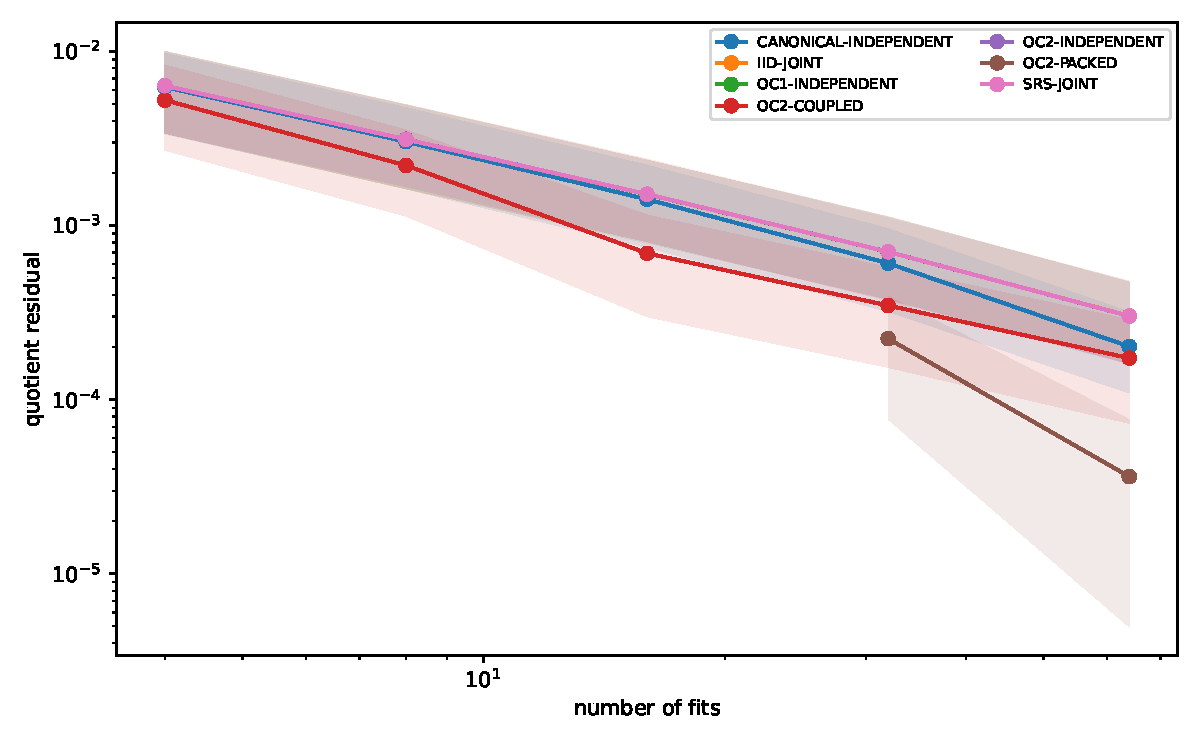
\includegraphics[width=.88\linewidth]{../../final_closure/figures/figure_1_independent_seed_showdown.pdf}
  \caption{Frozen $B=16$ independent-seed showdown across 144 neural cells.
  Residual is measured to each method's declared reference; Section
  \ref{sec:targetshift} audits the target difference.}
  \label{fig:showdown}
\end{figure}

At $B=16$, OC2-coupled has lower residual than canonical-independent in
144/144 cells and all 12 dataset means (Figure~\ref{fig:showdown}). The
equal-dataset reduction is 55.9\%, the median cell reduction is 72.4\%, and
the dataset-clustered 95\% interval is [38.7\%, 73.8\%]. Architecture
reductions are 93.2\% for MLP, 58.1\% for ResNet, 39.1\% for
FT-Transformer, and 90.2\% for TabM.

\begin{table}[t]
\centering
\caption{The frozen $B=16$ showdown. The residual column is method-relative;
the comparison is computational, not a same-estimand risk ordering.}
\label{tab:showdown}
\small
\begin{tabular}{lrrr}
\toprule
Method & Mean residual & Ratio to canonical & Wins \\
\midrule
OC2-coupled          & 0.000693 & 0.490 & 144/144 \\
Canonical-independent & 0.001415 & 1.000 & --- \\
OC1-independent     & 0.001512 & 1.068 & 7/144 \\
IID-joint           & 0.001513 & 1.069 & 2/144 \\
OC2-independent     & 0.001514 & 1.070 & 5/144 \\
SRS-joint           & 0.001514 & 1.070 & 7/144 \\
\bottomrule
\end{tabular}
\end{table}

\subsection{Symmetrization changes the target}
\label{sec:targetshift}

The mean squared distance between canonical and
schema$\times$independent expectations is $2.632\times10^{-4}$ (median
$1.005\times10^{-4}$), exceeding the cell-specific 95\% Monte Carlo threshold
in 10/144 cells. The finite coupled target is farther from the canonical target
on average ($2.494\times10^{-3}$). OrbitCover changes both what is averaged
and how efficiently that average is estimated. We therefore never infer
same-target dominance from Table~\ref{tab:showdown}.

\begin{figure}[t]
  \centering
  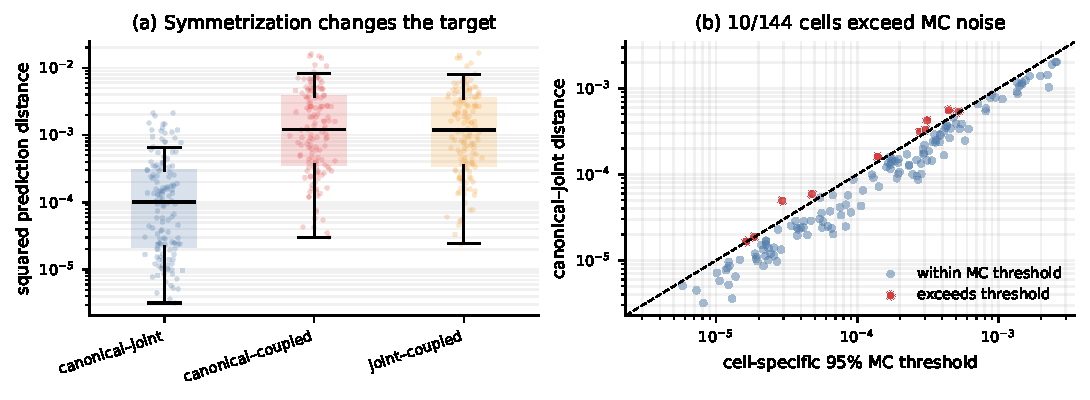
\includegraphics[width=.90\linewidth]{figures/target_shift_summary.pdf}
  \caption{Target shift. Left: cellwise target distances. Right: the
  canonical-to-joint distance against its cell-specific Monte Carlo threshold.}
  \label{fig:targets}
\end{figure}

\subsection{Joint balance, rather than schema balance alone, drives the gain}

OC2-independent beats canonical-independent in only 5/144 cells and no dataset
mean. Its equal-dataset reduction is $-7.0$\%, with a 95\% interval of
[$-7.8$\%, $-6.3$\%]. The same-target ablation gives the mechanism:
all-factor strength-2 balance has a mean cellwise residual reduction of 47.6\%
and wins 48/48 cells. Schema alone reduces residual by 13.0\%,
initialization alone by 7.0\%, and schema$\times$initialization balance by
34.0\%; all factors have the lowest residual. Schema$\times$initialization
fANOVA mass (0.01390) exceeds schema-only mass (0.00481), while joint
higher-order mass (0.01155) remains material.

\begin{figure}[t]
  \centering
  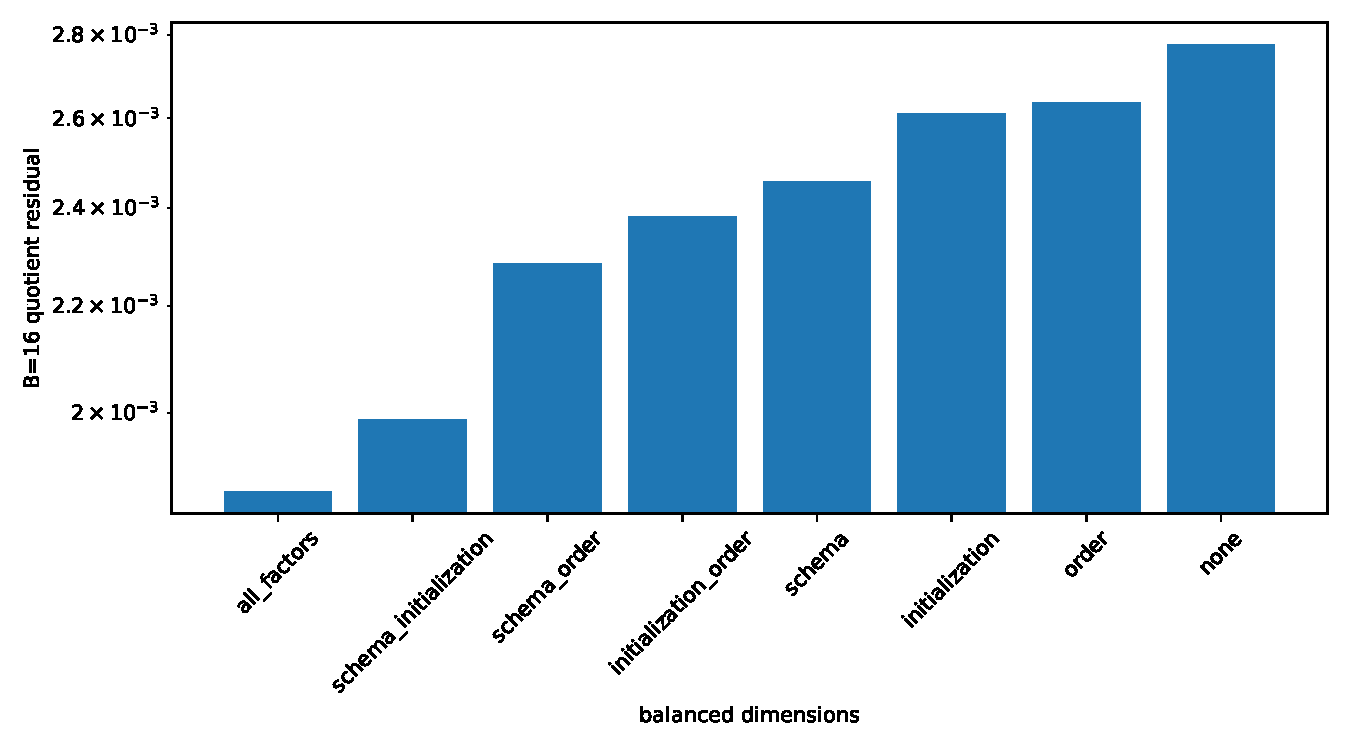
\includegraphics[width=.77\linewidth]{../../final_closure/figures/figure_10_coupling_mechanism.pdf}
  \caption{Same-target coupling ablation over 48 prospectively specified
  cells. Joint balance is not equivalent to schema balance plus arbitrary
  seeds.}
  \label{fig:coupling}
\end{figure}

\subsection{The benefit is finite-budget and interaction-dependent}

At convergence, the mean OC2/SRS residual ratio is 1.002: the strength-2
advantage does not persist on average. Nuisance variance remains nonzero, but
its useful coupling changes with architecture and training. Main+pair
fraction is only weakly associated with gain (Spearman $\rho=0.139$,
clustered interval [$-0.017$, 0.320]); higher-order fraction has
$\rho=0.258$ [0.038, 0.415]. Strength 3 recovers none of seven designated
strength-2/SRS losses. Interaction order is a boundary condition, not a
reliable per-cell oracle.

\begin{figure}[t]
  \centering
  \begin{minipage}[t]{.49\linewidth}
    \centering
    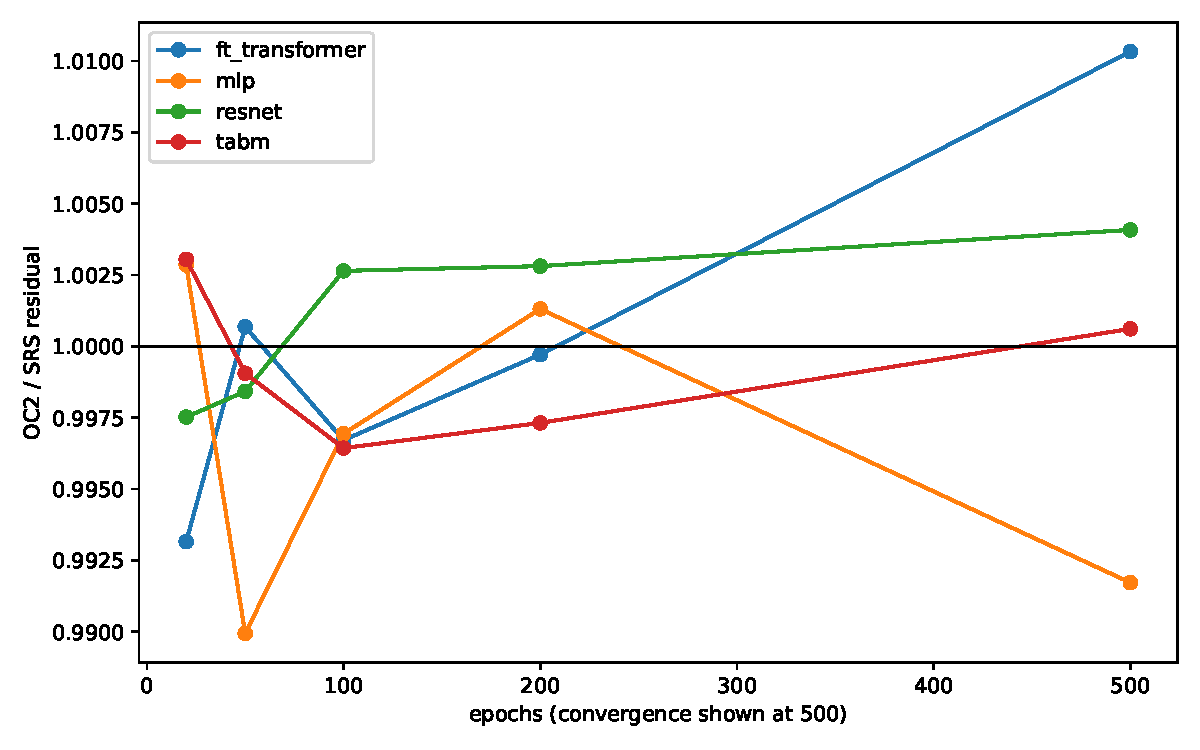
\includegraphics[width=\linewidth]{../../final_closure/figures/figure_6_orbitcover_convergence.pdf}
    \small (a) Relative efficiency at convergence.
  \end{minipage}
  \hfill
  \begin{minipage}[t]{.49\linewidth}
    \centering
    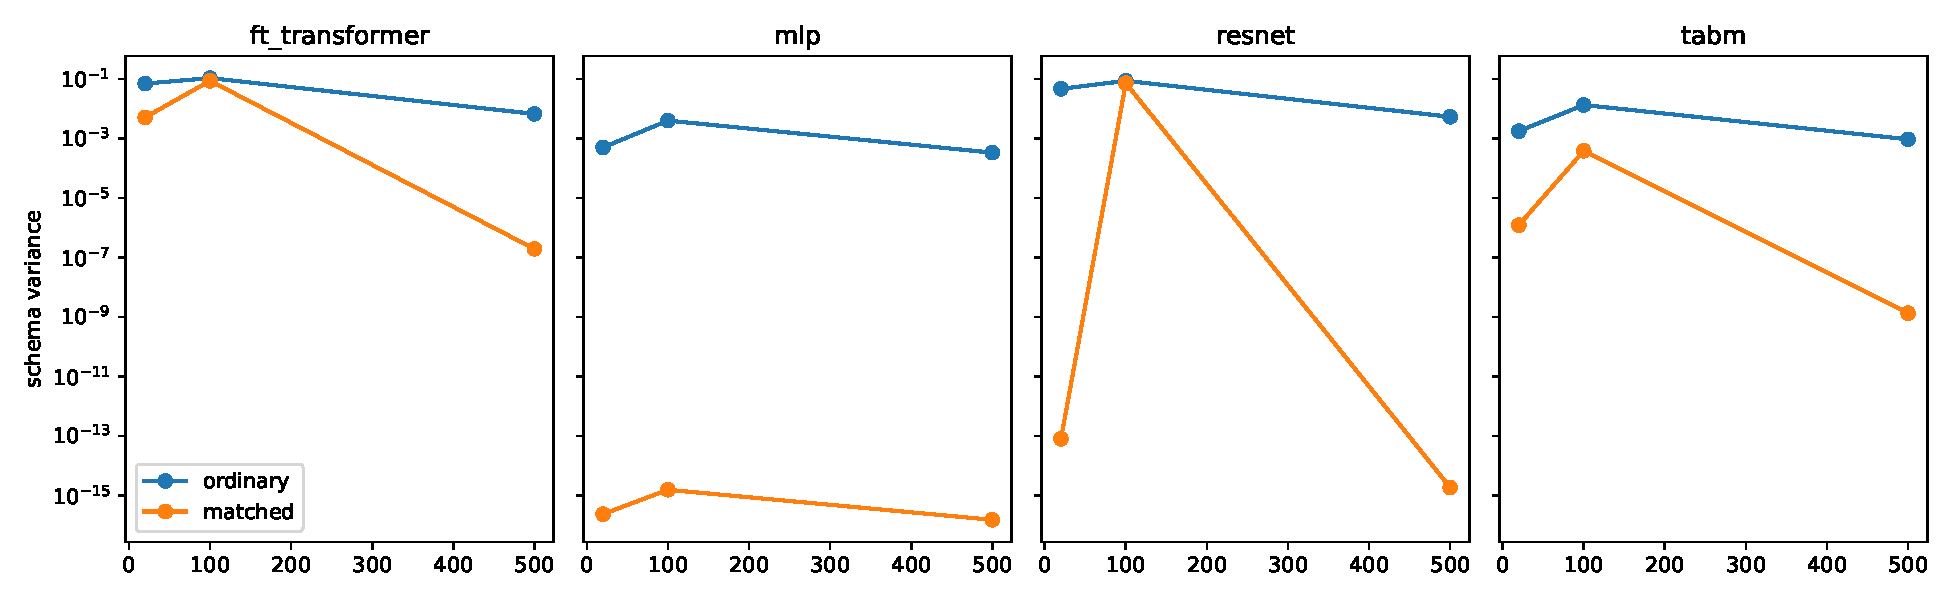
\includegraphics[width=\linewidth]{../../final_closure/figures/figure_9_matched_convergence.pdf}
    \small (b) Exact matched-function residual.
  \end{minipage}
  \caption{Training boundaries. The small-budget coupling effect is not a
  universal converged-path advantage.}
  \label{fig:convergence}
\end{figure}

\subsection{Exact matching narrows the optimizer-path claim}

Under exact transformed initialization, residual is effectively zero for MLP
($8.97\times10^{-16}$) and ResNet ($8.41\times10^{-14}$), but initially
remains 0.00262 for FT-Transformer and $4.19\times10^{-6}$ for TabM. At
convergence, the matched residual falls to $1.96\times10^{-7}$ and
$1.35\times10^{-9}$, respectively. Schema does not universally induce
irreducible optimizer-path divergence. Architecture-specific tokenization,
member structure, dropout, and minibatch dynamics remain the supported scope.

\subsection{Validation fidelity does not imply held-out selection gain}

In the prior exact selection panel, strength-2 winner agreement is 99.41\%
versus 96.69\% for IID, and rank correlation is 98.64\% versus 96.77\%.
Yet exact validation and test winners agree in only 19/36 partitions.
Held-out selected-test regret changes only from 0.005029 to 0.004906.
Partition shift dominates the remaining selection error; we claim no
practically meaningful held-out performance improvement.

\section{Related work}

\paragraph{Tabular models and evaluation.}
TabM \citep{gorishniy2025tabm} shows that efficient ensembles are strong
tabular baselines; we study which nuisance law such an ensemble integrates.
TabPFN-v2, TabDPT, and TabSTAR learn broad tabular priors or representations
\citep{hollmann2025tabpfn,ma2025tabdpt,arazi2025tabstar}. TabArena and TabReD
stress realistic benchmarking \citep{erickson2025tabarena,rubachev2025tabred}.
OrbitCover addresses variation inside a fixed data partition and does not
solve temporal or population shift.

\paragraph{Symmetrization and multiplicity.}
Metamorphic testing already treats attribute and class-label permutations as
valid supervised transformations \citep{xie2011metamorphic}. Frame averaging
and learned probabilistic symmetrization reduce or learn group averages
\citep{puny2022frame,kim2023probabilistic}. OrbitCover instead samples
complete retraining pipelines, returns an unbiased estimate rather than an
exactly invariant realized network, and includes stochastic training factors.
Neural training multiplicity itself is established
\citep{summers2021nondeterminism}; our focus is the product estimand.

\paragraph{Design and stable risk estimation.}
Randomized OAs and OA-based Latin hypercubes remove low-order ANOVA terms
\citep{owen1992oa,ai2016oa}. OAs have also constructed low-correlation
training ensembles \citep{johnson2021ensembles}, and orthogonal Monte Carlo
couples continuous samples \citep{choromanski2019omc}. Antithetic
cross-validation couples response perturbations and gives strong contemporary
risk theory \citep{liu2026antithetic,chattopadhyay2026optimal}. These works
rule out generic OA or antithetic novelty. OrbitCover acts on a finite
semantic-pipeline nuisance product without perturbing responses or changing
train/test membership.

\section{Limitations and conclusion}

The quotient is only as meaningful as its declared nuisance law. A uniform
finite menu is transparent, but deployment may require a nonuniform or robust
target. The 128-seed canonical and 512/1,024-fit joint references retain Monte
Carlo error. Dataset-clustered intervals describe this 12-source panel rather
than a distribution-free population. Evidence is tabular and limited to four
primary neural architectures.

Quadratic prediction residual is the endpoint justified by (2). Accuracy,
AUROC, calibration, fairness, and population-shift robustness can behave
differently. The method is not universal: OC2-independent fails, average
OC2/SRS efficiency vanishes at convergence, strength 3 does not repair the
designated failures, and exact function matching nearly closes MLP and ResNet.

Within that boundary, the positive result is broad and mechanistically
coherent. OrbitCover makes exact representation equivalences and training
randomness into a finite semantic quotient, exposes its prediction-space
interactions, and uses a coupled strength-2 design to estimate it efficiently
at small budget. The practical lesson is conditional: design randomization
around the interactions of the \emph{declared} pipeline, and audit both target
shift and finite-budget benefit.

\subsection*{AI use statement}

Generative AI tools (OpenAI Codex) were used for literature discovery,
hypothesis generation, confirmatory-protocol and experimental-code drafting,
statistical-analysis assistance, figure-script preparation, manuscript
drafting, and language editing. The authors selected and froze the
confirmatory protocols before their outcomes, executed the experiments,
inspected the generated artifacts, and checked the reported calculations and
citations against primary sources. All AI-assisted code is covered by the
reported tests and artifact audit. The authors take responsibility for the
final text, claims, code, and results.

\subsection*{Ethics statement}

This work uses established public tabular benchmarks and introduces no human-
subject data collection. Its main risk is evaluation overclaiming: an
unstated nuisance law could obscure model multiplicity, while inappropriate
symmetrization could waste compute or change a prediction target. We mitigate
this by releasing action menus, semantic-alignment checks, cross-target
distances, uncertainty, and all designated failures.

\subsection*{Reproducibility statement}

The supplement contains the frozen protocol and hashes, all recorded
deviations, model and dataset details, exact theorem statements, complete
failure inventories, and regeneration commands. Machine-readable cell tables,
summary JSON, vector PDF figures, and the persistent fit registry accompany
the source. A read-only audit verifies 140,592 unique fit keys, 1,128 aligned
prediction arrays, 125,616 independent seed records, all mandatory manifests,
and 116/116 tests.

\bibliography{references}
\bibliographystyle{iclr2027_conference}

\appendix
\section{Proof details}

\paragraph{Quadratic ambiguity identity.}
Write $Y-P_Z=(Y-Q_\mu)+(Q_\mu-P_Z)$, expand the squared Hilbert norm, and take
expectations. The cross term is zero because $\E(P_Z-Q_\mu)=0$, proving (2).
The same argument with $\Qhat_{\mathcal D}$ shows that cover residual is exact
expected Brier/MSE overhead whenever the design is unbiased for $Q_\mu$.

\paragraph{Product fANOVA filter.}
Define $f_u$ recursively by subtracting every lower-order conditional
expectation from $\E[P_Z\mid Z_u]$. Under a product measure these components
are mutually orthogonal. Randomized factor-label permutations make the design
covariance commute with each factor's symmetric-group action, so it is scalar
on each tensor-product contrast subspace. Projection and trace normalization
give (4). Strength $t$ makes every empirical marginal through order $t$
uniform, hence annihilates those subspaces.

\section{Additional experimental details}

\paragraph{Architectures.}
All primary cells use the frozen MLP, ResNet, FT-Transformer, and TabM widths,
AdamW, batch size 256, learning rate $10^{-3}$, weight decay $10^{-4}$, and
20 epochs unless the scale experiment explicitly changes the budget. The
convergence arm uses at most 500 epochs, patience 30, relative minimum
improvement $10^{-4}$, and restores the best checkpoint.

\paragraph{Reference construction.}
Every fit is keyed by dataset, split, model/configuration hash, schema hash,
master RNG seed or declared finite init/order pair, training size, budget, and
matched arm. Prediction files are registered only after shape, alignment, and
finiteness checks. Resampling uses 512 deterministic estimator draws per cell
and method; overlaps are never counted as independent evidence.

\paragraph{Compute.}
The audited registry represents 140,592 fits and 232.005 summed local fit-hours
(231.802 GPU and 0.203 CPU). These measurements document execution and
reproducibility, not portable latency, energy, or monetary speedup.

\section{Complete headline ledger}

\begin{table}[h]
\centering
\small
\begin{tabular}{p{.48\linewidth}p{.40\linewidth}}
\toprule
Claim & Audited value \\
\midrule
OC2-coupled vs canonical-independent &
144/144 cell wins; 12/12 dataset wins; 55.9\% [38.7\%, 73.8\%] \\
OC2-independent vs canonical-independent &
5/144 cell wins; 0/12 dataset wins; $-7.0$\% [$-7.8$\%, $-6.3$\%] \\
Canonical-to-independent-joint distance &
Mean $2.632\times10^{-4}$; 10/144 over cellwise MC threshold \\
Same-target all-factor ablation &
48/48 wins; 47.6\% mean cellwise reduction \\
Convergence boundary &
Mean OC2/SRS residual ratio 1.001683 \\
Interaction prediction &
Main+pair $\rho=.139$ [$-.017,.320$]; higher $\rho=.258$ [.038,.415] \\
Selection boundary &
Exact validation/test winner agreement 19/36; regret .005029 to .004906 \\
\bottomrule
\end{tabular}
\end{table}

\section{Excluded claims}

The evidence does not support universal superiority over independent seed
ensembling, a common expectation across methods, persistent convergence
efficiency, universal irreducible optimizer-path dependence, strength-3
dominance, meaningful held-out accuracy improvement, or portable systems
speedup. OAs, fANOVA filtering, group averaging, antithetic dependence, and
proper-score variance identities are cited as prior art rather than claimed
as inventions.

\end{document}
